\section*{Hardware}

Regarding the hardware used in this project, Figure~\ref{fig:circuit} shows a complete overview of which elements have been used and how they were connected.
\begin{figure}[h]
    \centering
    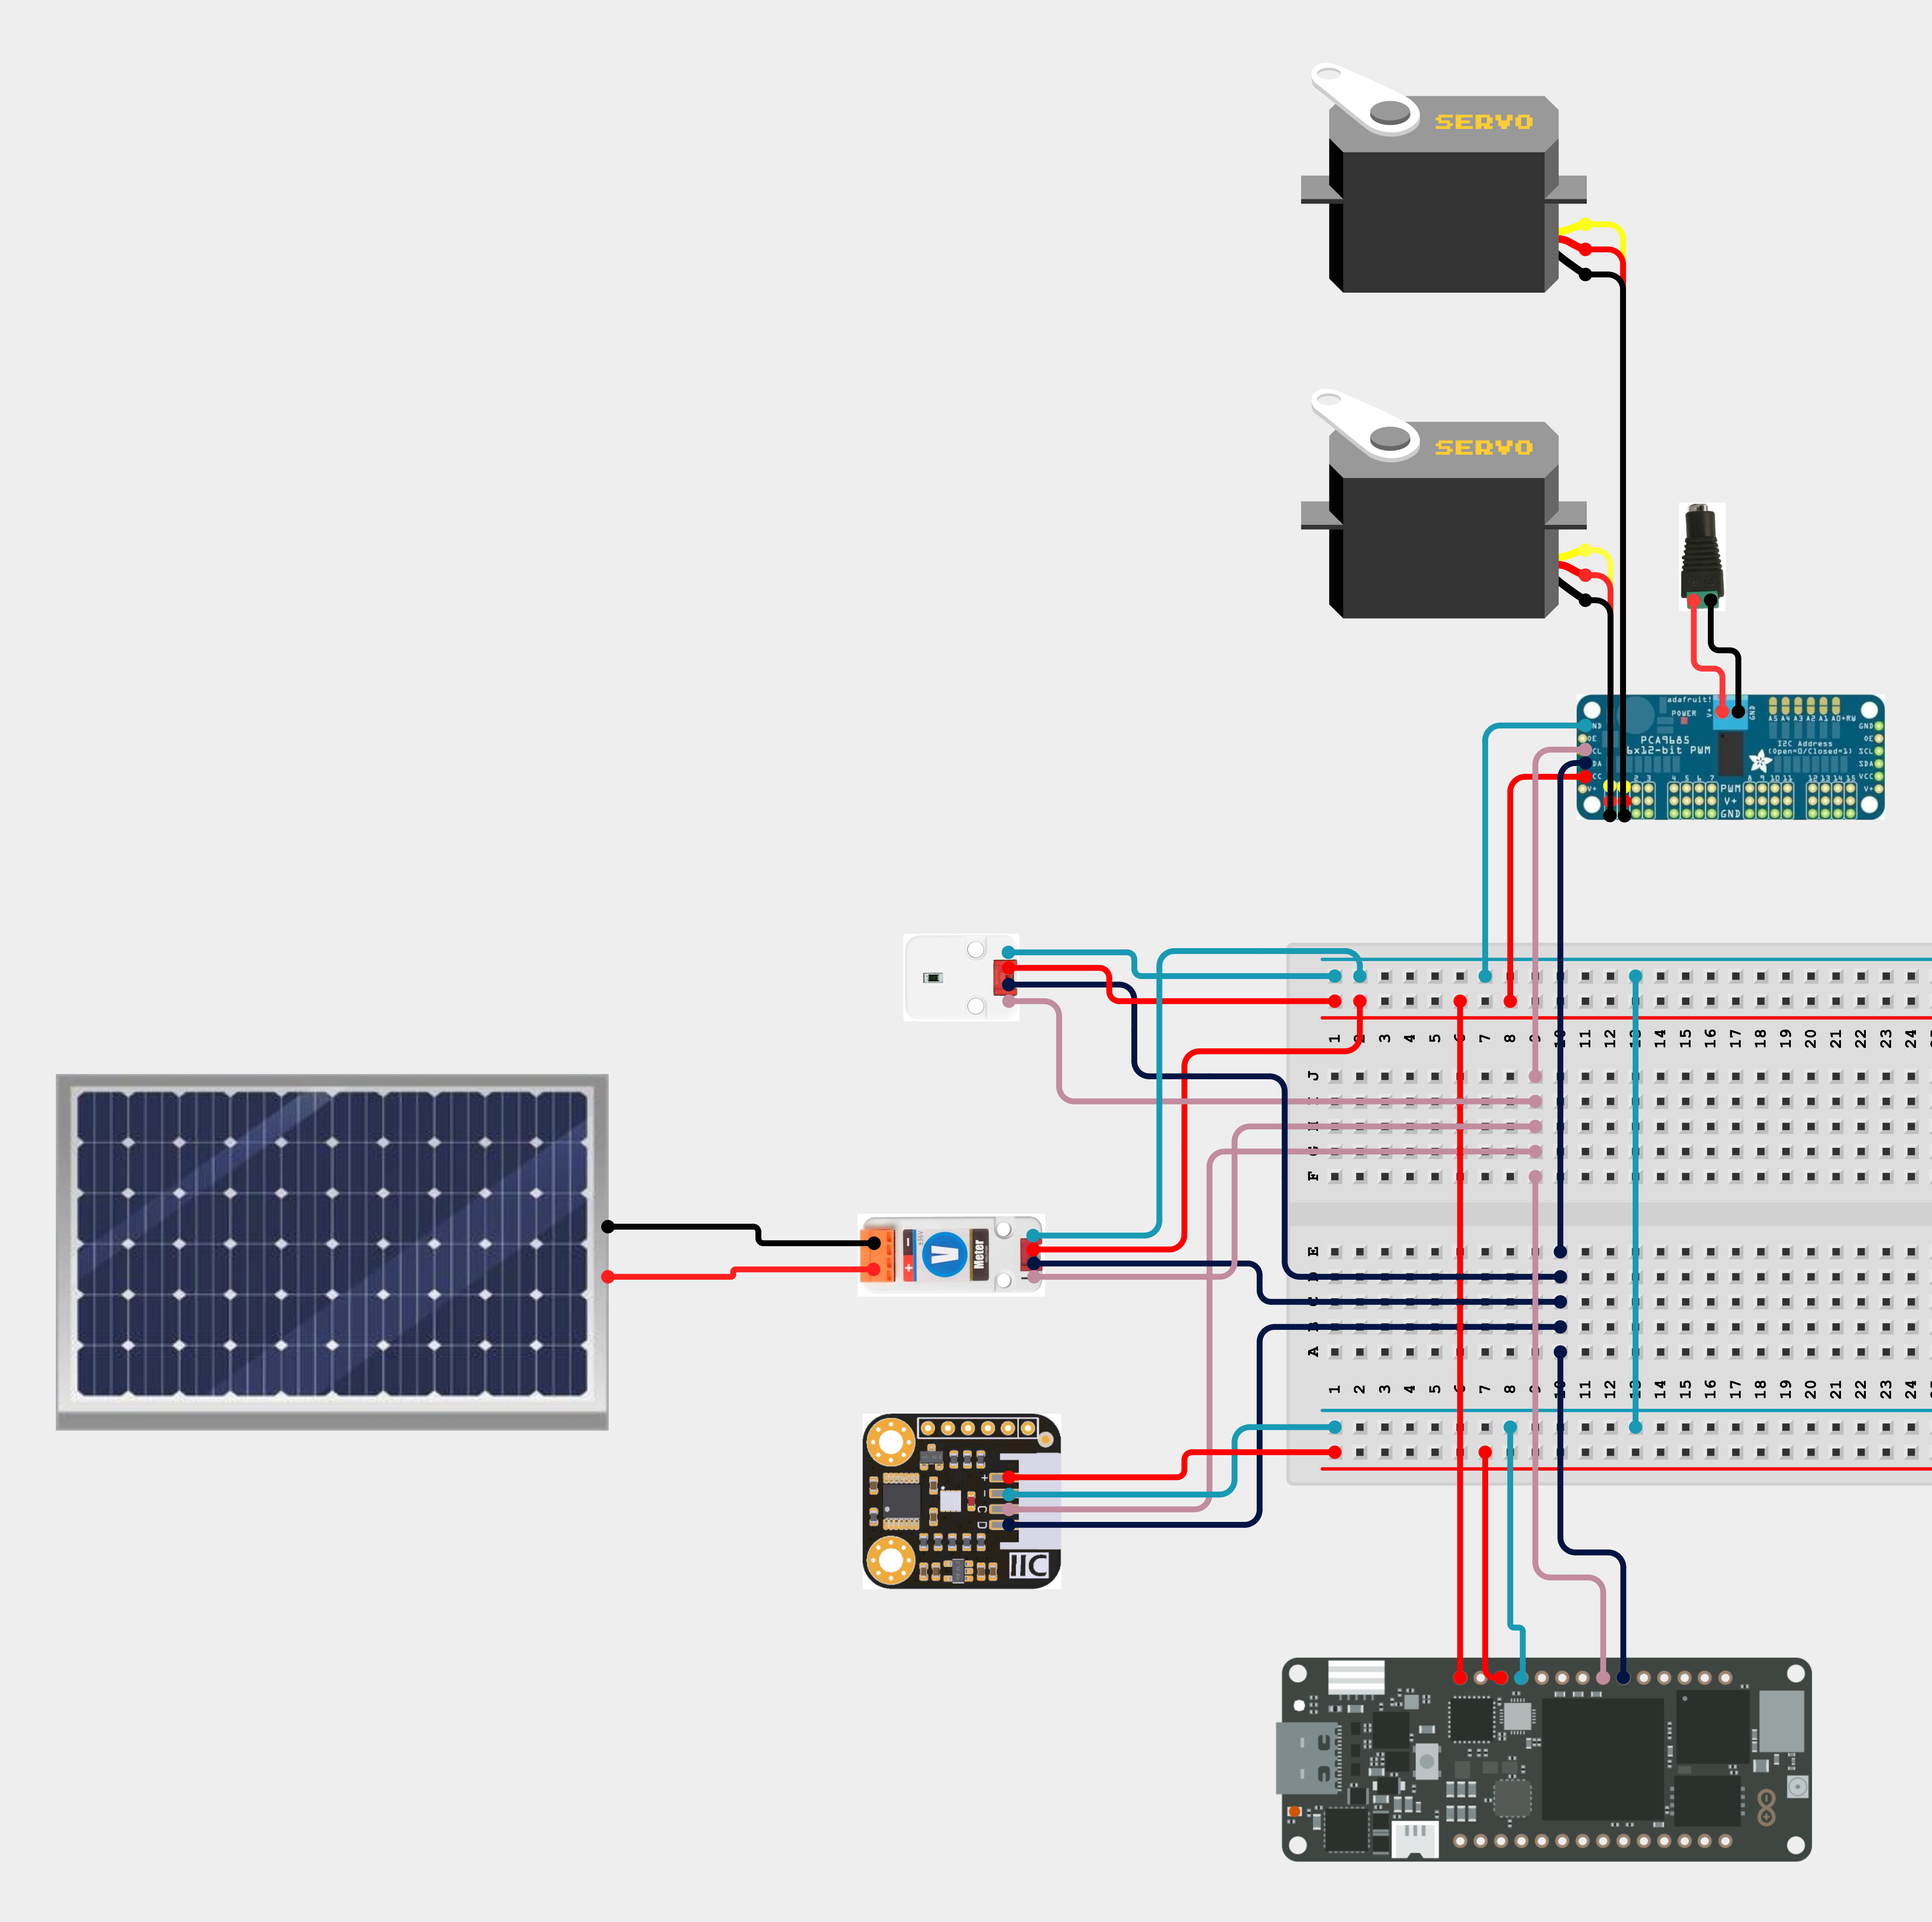
\includegraphics[width=10cm]{../assets/png/project-circuit}
    \caption{Overview of the hardware used in our project.}
    \label{fig:circuit}
\end{figure}
The parts used where: two servos, a motor shield, a light intensity sensor, a voltmeter connected to a solar panel, an ambient sensor, and an Arduino Portenta H7.
All the components were connected to the Portenta board using the I2C protocol.

\subsection*{Servos}
The two servos are the responsible for the movement of the solar panel.
These are high-torque servos and are attached to a 3D-printed structure that holds the solar panel and moves it on two different planes.
The bottom servo rotates the panel, while the top servo adjusts the inclination of the panel. \\ \\
To be able to interface with the Arduino board, we used a motor shield to which we connected both servos.
Since they require some energy, the shield was connected to the wall outlet by means of a power supply cable.

\subsection*{Ambient Sensor}
Attached to the system, there is an ambient sensor which will capture several different measurements.
These measurements are temperature, pressure, humidity, and light intensity.
These measurements are not used to drive the best-position-seeking algorithm for the solar panel, but are used to populate the weather station's dashboard.

\subsection*{Light Intensity Sensor}
As with the ambient sensor, the light intensity sensor does not serve a real purpose towards the computation of the best position.
The data taken from this sensor is used in the weather station dashboard.

\subsection*{Voltmeter}

The system must actively adjust the solar panel in response to the position of the sun, adjusting its position to maximize energy absorption.
This is done with two main actions, searching for the optimal position and scanning the various positions and angles. \\ \\
Our model must also take into account times of low solar intensity such as cloudy conditions or night.
In these scenarios, our system enters an energy-saving phase.
The system will only capture sensor data, and as long as the produced voltage does not exceed 1V, the system will not search for new positions (Figure~\ref{fig:seros-sm}).
\begin{figure}[h]
    \centering
    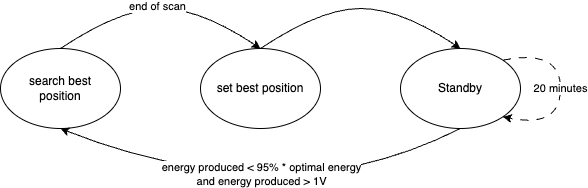
\includegraphics[width=12cm]{../assets/png/servos-state-machine}
    \caption{State machine that describes the lifecycle of our system.}
    \label{fig:seros-sm}
\end{figure}
